% Fig. 3.13 -- the stretch of the range on which a truncated distribution
%   lives.
% Source: mathstatch3.tex lines 1520-1552.
%
% The manuscript draws the schematic curve 2 e^{-(x-3)^2/2} over 0 <= x <= 6,
% shades it between a = 1.6 and b = 4.4, drops a dashed boundary from the
% curve to the axis at each of the two, labels those two a and b, and writes
% P(a<X<b) inside the shaded block.  Per CH2_FIGURE_SPECS.md 1.6 the web
% version puts a genuine density in its place,
%   f_X(x) = 0.3989423 e^{-(x-3)^2/2},
% which integrates to 1, so that the shaded block really is the probability
% its label names.
%
% This figure and truncated-normalized.tex (Fig. 3.14) are read against each
% other: the second one is the first one divided by P(a<X<b), and the whole
% point of the pair is that the curve stands higher in the second.  For the
% comparison to hold on the page the two have to render at one scale, and
% since an SVG is fitted to the column width, that means the two drawings
% must be exactly as wide as each other.  Both therefore carry the same
% invisible \path across the foot of the picture, which fixes the left edge,
% the right edge and the floor; the top is left to find its own level, so
% neither picture carries a band of empty space above its curve.
%
% Boundaries: a = 2.0 and b = 4.4, not the manuscript's symmetric 1.6 and
% 4.4.  Two reasons.  An interval placed off-centre reads as a general
% interval rather than as something tied to the peak (the same move is
% recorded for Fig. 2.11 in continuous-interval-area.tex), and
%   P(2.0 < X < 4.4) = 0.7605876,
% so Fig. 3.14 lifts the curve by 1/0.7605876 = 1.3147721, a lift the eye
% can see.  At the manuscript's 1.6 and 4.4 the probability is 0.8384866 and
% the lift only 1.1926, which at this scale is 0.6cm at the peak and reads
% as a drawing accident rather than as the point of the figure.
%
% Drawing scale x = 1.05cm, y = 6.4cm.  Heights: peak 2.55323cm,
% f_X(a) = 1.54861cm, f_X(b) = 0.95826cm.  Over the plotted range
% 0 <= x <= 6.2 the curve encloses 0.997963 rather than 1, the remainder
% being the two tails outside the range.
%
% Deviations from the manuscript picture:
%
% 1. The curve is labelled f_X(x) above its peak.  The manuscript has that
%    label in the source but commented out, so its picture leaves the curve
%    unnamed; without the name here, the f_X(x|a<X<b) of Fig. 3.14 has
%    nothing to be read against.
%
% 2. \DeclareMathSizes{10}{10}{9}{8} raises the math script sizes from the
%    default 7pt/5pt, as CH2_FIGURE_SPECS.md 1.3 requires wherever \sssig
%    appears.  Native size 221.82 x 112.945 pt (drawing 7.65cm wide, shared
%    with Fig. 3.14).  A mark of S pt shows at
%    S x 0.99626 x <display width> / 221.82 px, so at the 350px phone width
%    of a topic-figure--wide in body text
%        10pt text 15.72px, 9pt scripts 14.15px, 8pt scriptscripts 12.58px
%    and at the 620px desktop width 27.85 / 25.06 / 22.28px.
\documentclass[tikz,border=2pt]{standalone}
\usepackage{amsmath}
\usepackage{amssymb}
\usepackage{xcolor}
\usetikzlibrary{arrows.meta}
\newcommand{\sssig}{\scriptscriptstyle}
\DeclareMathSizes{10}{10}{9}{8}

\definecolor{journalink}{HTML}{1F1C18}
\definecolor{journalmuted}{HTML}{8A7F72}
\definecolor{journalaccent}{HTML}{9C2D2D}

\begin{document}
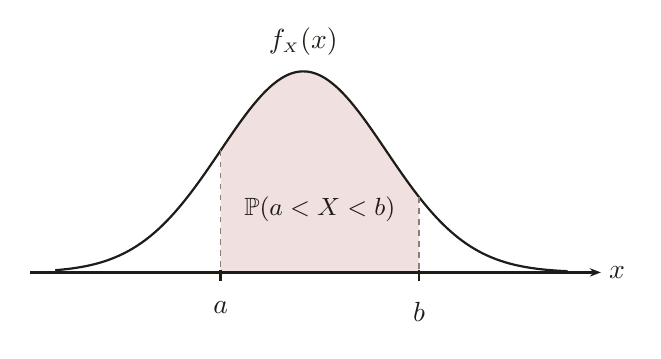
\begin{tikzpicture}[
  x=1.05cm,
  y=6.4cm,
  every node/.style={font=\normalsize, journalink},
  axis/.style={journalink, line width=0.8pt, -{Stealth[length=4pt]}},
  tick/.style={journalink, line width=0.8pt},
  curve/.style={journalink, line width=0.8pt},
  guide/.style={journalmuted, line width=0.5pt, dash pattern=on 2pt off 2pt},
  region/.style={journalaccent, fill opacity=0.15}
]
  % ---- left edge, right edge and floor, shared with Fig. 3.14 ----------
  \path (-0.35cm,-0.70cm) -- (7.30cm,-0.70cm);

  % ---- the block between a and b --------------------------------------
  \fill[region]
    (2.0,0) -- (4.4,0) -- (4.4,0.1497275)
    -- plot[domain=4.4:2.0, samples=200, smooth]
       (\x,{0.3989423*exp(-(\x-3)*(\x-3)/2)})
    -- cycle;

  % ---- density curve ---------------------------------------------------
  \draw[curve] plot[domain=0:6.2, samples=200, smooth]
    (\x,{0.3989423*exp(-(\x-3)*(\x-3)/2)});

  % ---- x axis ----------------------------------------------------------
  \draw[axis] (-0.3,0) -- (6.6,0);
  \node[anchor=west, inner sep=2.8pt] at (6.6,0) {$x$};

  % ---- the two boundaries ----------------------------------------------
  \draw[guide] (2.0,0.2419707) -- (2.0,0);
  \draw[guide] (4.4,0.1497275) -- (4.4,0);
  \draw[tick] ([yshift=0.035cm]2.0,0) -- ([yshift=-0.106cm]2.0,0);
  \draw[tick] ([yshift=0.035cm]4.4,0) -- ([yshift=-0.106cm]4.4,0);
  \node[anchor=north] at ([yshift=-0.25cm]2.0,0) {$a$};
  \node[anchor=north] at ([yshift=-0.25cm]4.4,0) {$b$};

  % ---- the probability of the block ------------------------------------
  % At 0.80cm the curve stands above the label for 1.476 < x < 4.524, so at
  % that height both edges of the block are the two boundaries themselves
  % and the block is centred on x = 3.2.  The label is set \small, as the
  % manuscript sets it, which leaves 0.30cm between it and each boundary.
  \node[inner sep=0pt] at ([yshift=0.80cm]3.2,0)
    {\small $\mathbb{P}(a<X<b)$};

  % ---- curve label -----------------------------------------------------
  \node[anchor=south, inner sep=0pt] at ([yshift=2.75cm]3.0,0)
    {$f_{\sssig X}(x)$};
\end{tikzpicture}
\end{document}
